\documentclass[11pt]{article}

\usepackage[margin=1in]{geometry}
\usepackage{graphicx}
\usepackage{amsmath}
\usepackage{float}

\title{CTA200 Assignment 3 Results}
\author{Alexis Li}
\date{May 12, 2026}

\begin{document}

\maketitle

\section{Question 1: Mandelbrot Iteration}

For Question 1, I investigated the iteration
\[
z_{i+1}=z_i^2+c,
\]
with initial value \(z_0=0\). The complex number \(c\) was constructed from points
\((x,y)\), where \(x\) was used as the real component and \(y\) was used as the
imaginary component. For each point, I iterated the equation up to 1000 times and
defined divergence as the condition \(|z|>2\).

Figure \ref{fig:mandelbrot_points} shows the points in the complex plane that
diverged under this iteration. Figure \ref{fig:mandelbrot_iterations} shows the
number of iterations required for divergence, using a logarithmic colour scale.

\begin{figure}[H]
    \centering
    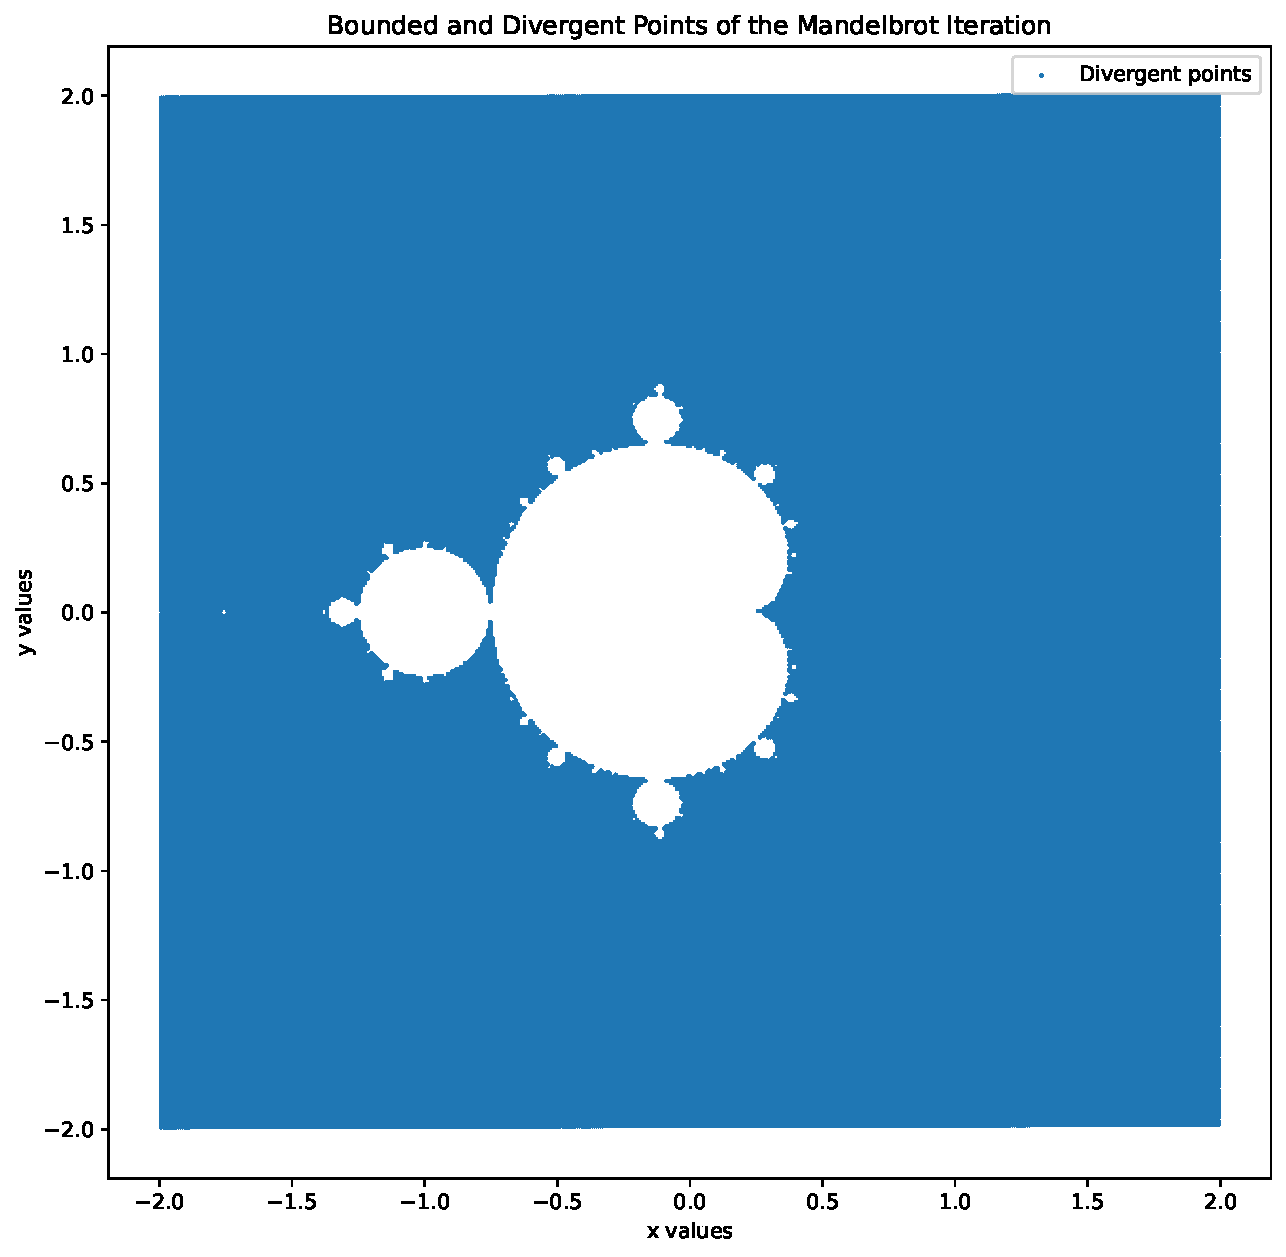
\includegraphics[width=0.7\textwidth]{mandelbrot_points.pdf}
    \caption{Points in the complex plane that diverged under the Mandelbrot iteration.}
    \label{fig:mandelbrot_points}
\end{figure}

\begin{figure}[H]
    \centering
    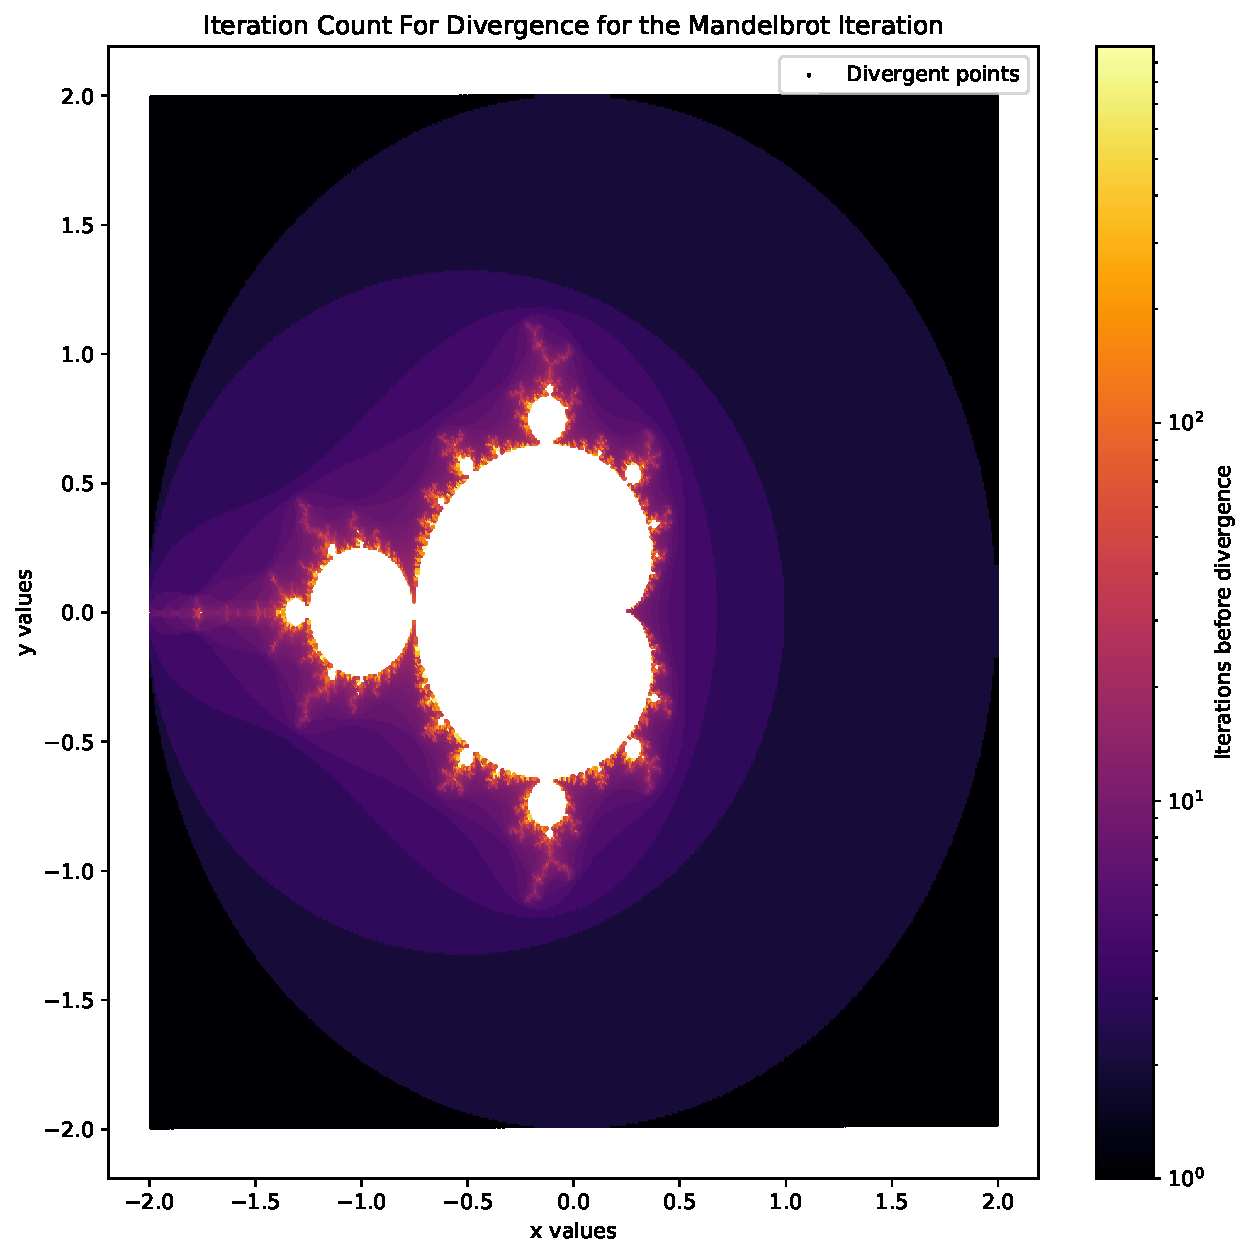
\includegraphics[width=0.7\textwidth]{mandelbrot_iterations.pdf}
    \caption{Iteration count required for divergence in the Mandelbrot iteration.}
    \label{fig:mandelbrot_iterations}
\end{figure}

\section{Question 2: Lorenz System}

For Question 2, I solved the Lorenz system
\[
\frac{dX}{dt}=-\sigma(X-Y),
\]
\[
\frac{dY}{dt}=rX-Y-XZ,
\]
\[
\frac{dZ}{dt}=-bZ+XY.
\]
I used the parameter values
\[
\sigma=10, \qquad r=28, \qquad b=\frac{8}{3},
\]
with Lorenz's initial condition
\[
W_0=[0,1,0].
\]
The system was integrated numerically using \texttt{solve\_ivp} from \(t=0\) to
\(t=60\). Dense output was used so that the solution could be evaluated at closely
spaced time values for plotting.

Figure \ref{fig:lorenz_fig1} reproduces Lorenz's Figure 1 by plotting \(Y\) against
the iteration number
\[
N=\frac{t}{\Delta t},
\]
where \(\Delta t=0.01\). The three panels show the intervals \(N=0\) to \(1000\),
\(N=1000\) to \(2000\), and \(N=2000\) to \(3000\).

\begin{figure}[H]
    \centering
    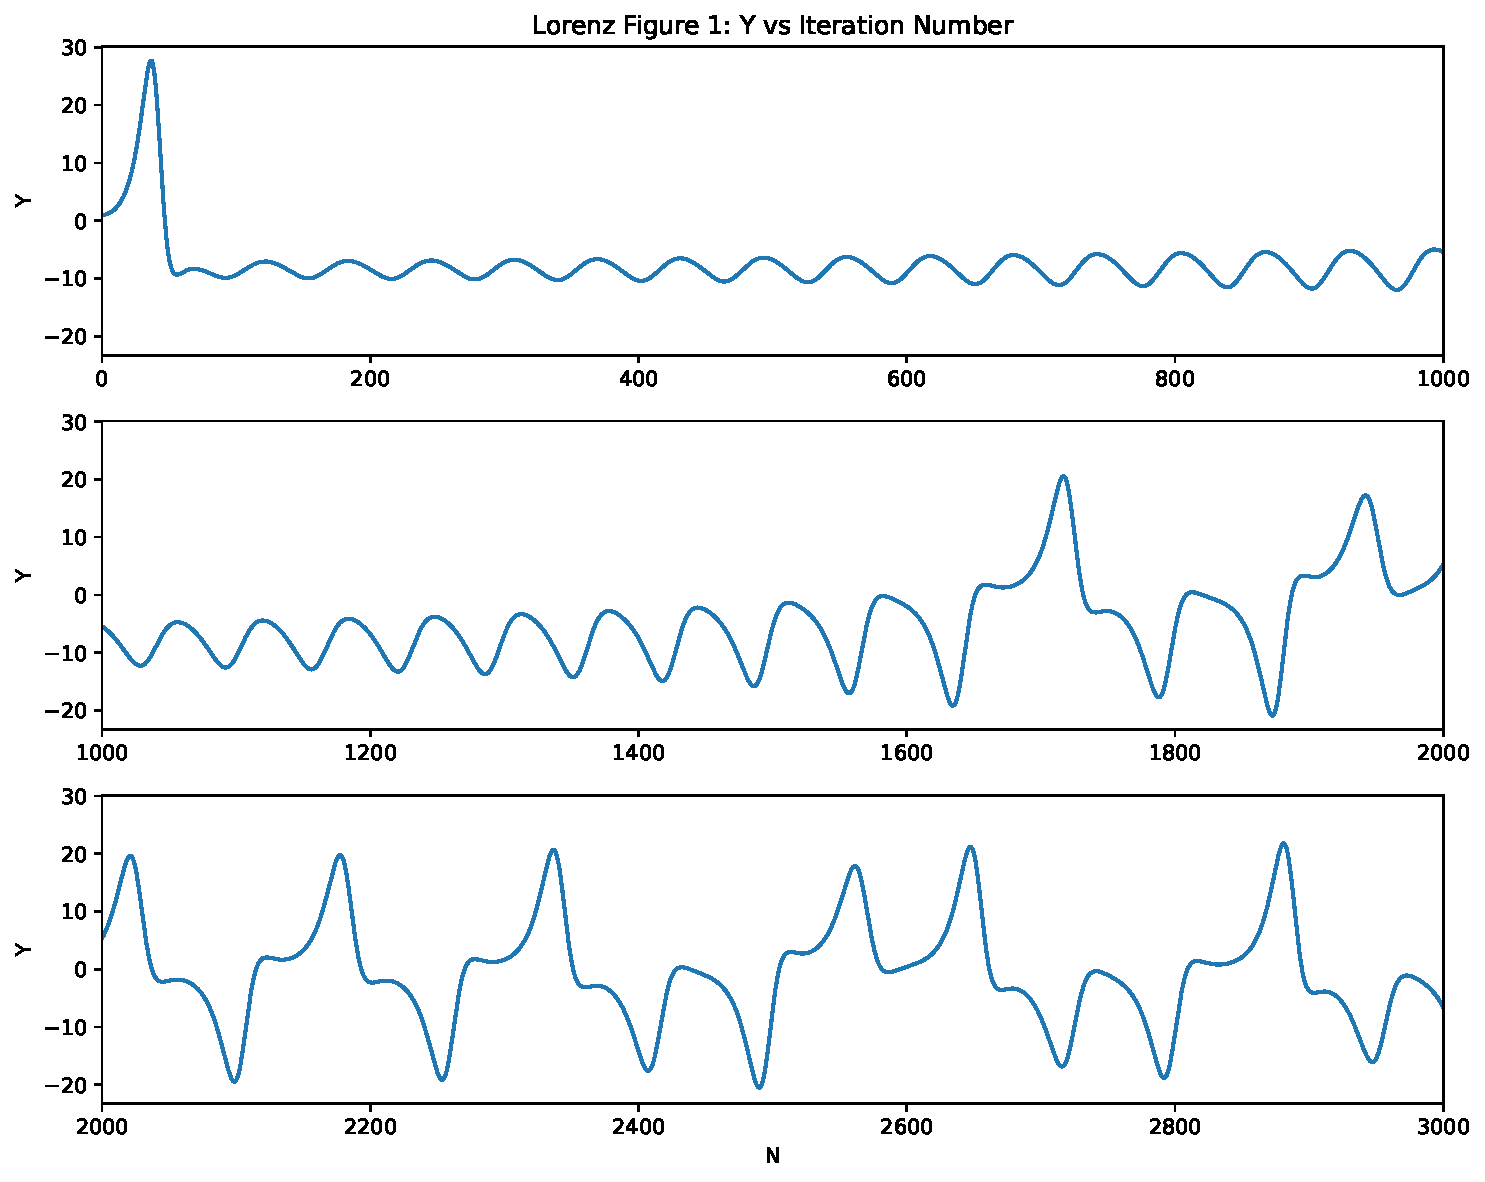
\includegraphics[width=0.85\textwidth]{lorenz_fig1.pdf}
    \caption{Reproduction of Lorenz's Figure 1, showing \(Y\) as a function of iteration number \(N\).}
    \label{fig:lorenz_fig1}
\end{figure}

Figure \ref{fig:lorenz_fig2} reproduces Lorenz's Figure 2. The solution was
evaluated for \(14\leq t\leq 19\), corresponding to \(1400\leq N\leq 1900\). The
top panel shows the projection onto the \(Y\)-\(Z\) plane, while the bottom panel
shows the projection onto the \(Y\)-\(X\) plane.

\begin{figure}[H]
    \centering
    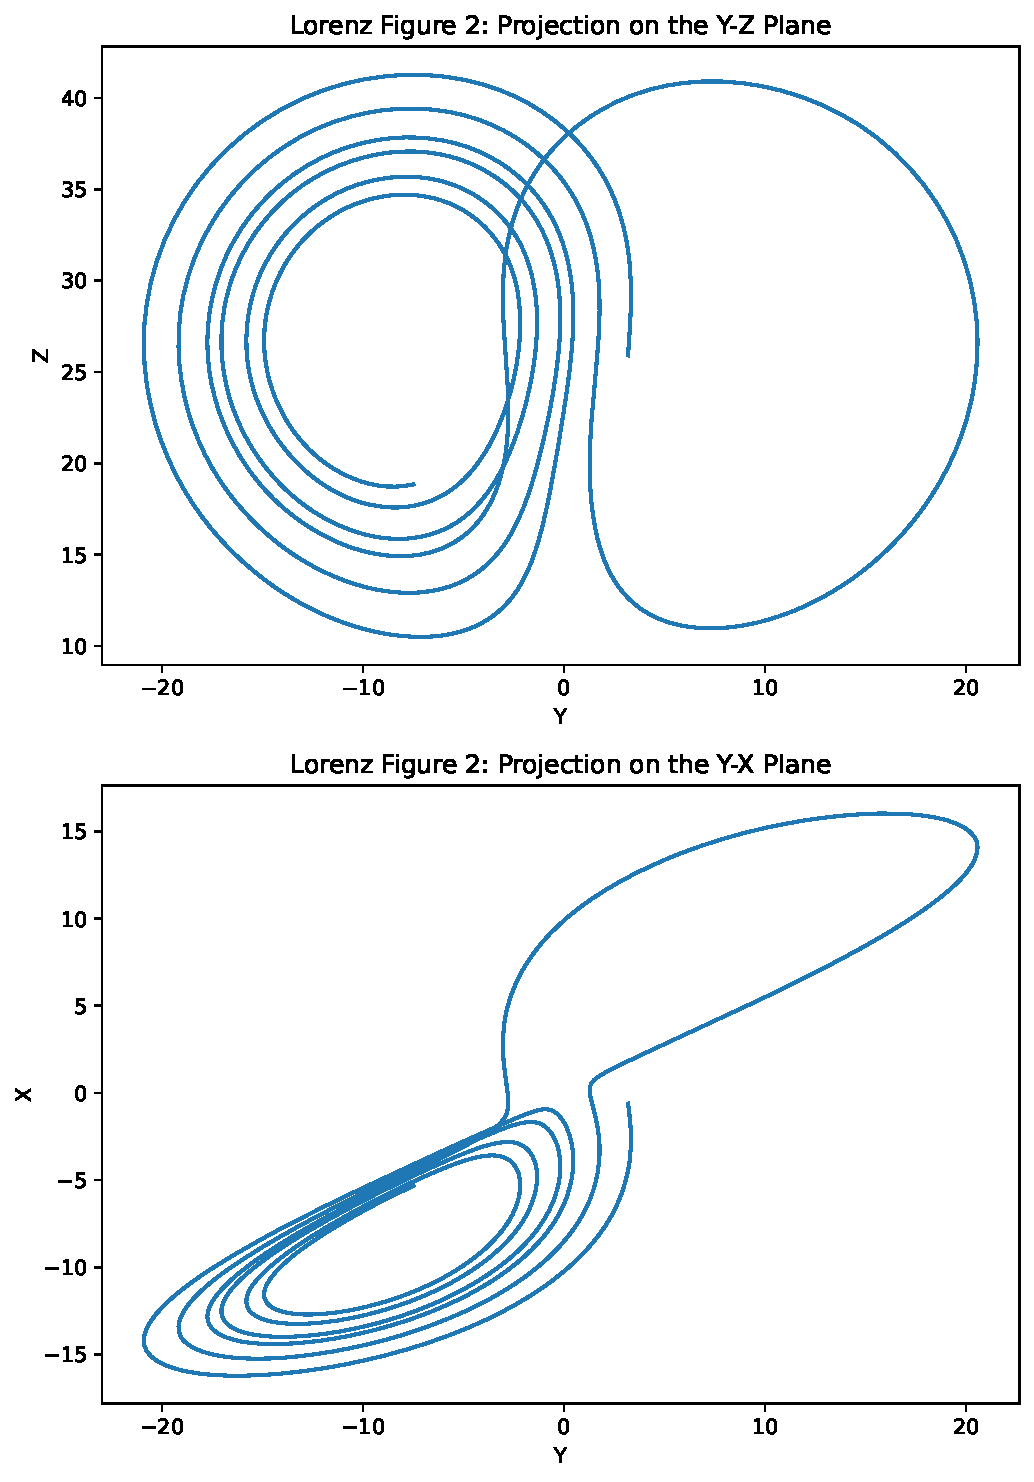
\includegraphics[width=0.75\textwidth]{lorenz_fig2.pdf}
    \caption{Reproduction of Lorenz's Figure 2, showing projections of the Lorenz trajectory.}
    \label{fig:lorenz_fig2}
\end{figure}

To investigate the sensitivity of the system to initial conditions, I solved the Lorenz system again using
the slightly preturbed initial condition
\[
W_0'=[0,1.00000001,0].
\]
I then calculated the distance between the original and perturbed solutions:
\[
d(t)=\sqrt{(X'-X)^2+(Y'-Y)^2+(Z'-Z)^2}.
\]
The result is shown in Figure \ref{fig:lorenz_divergence}.

\begin{figure}[H]
    \centering
    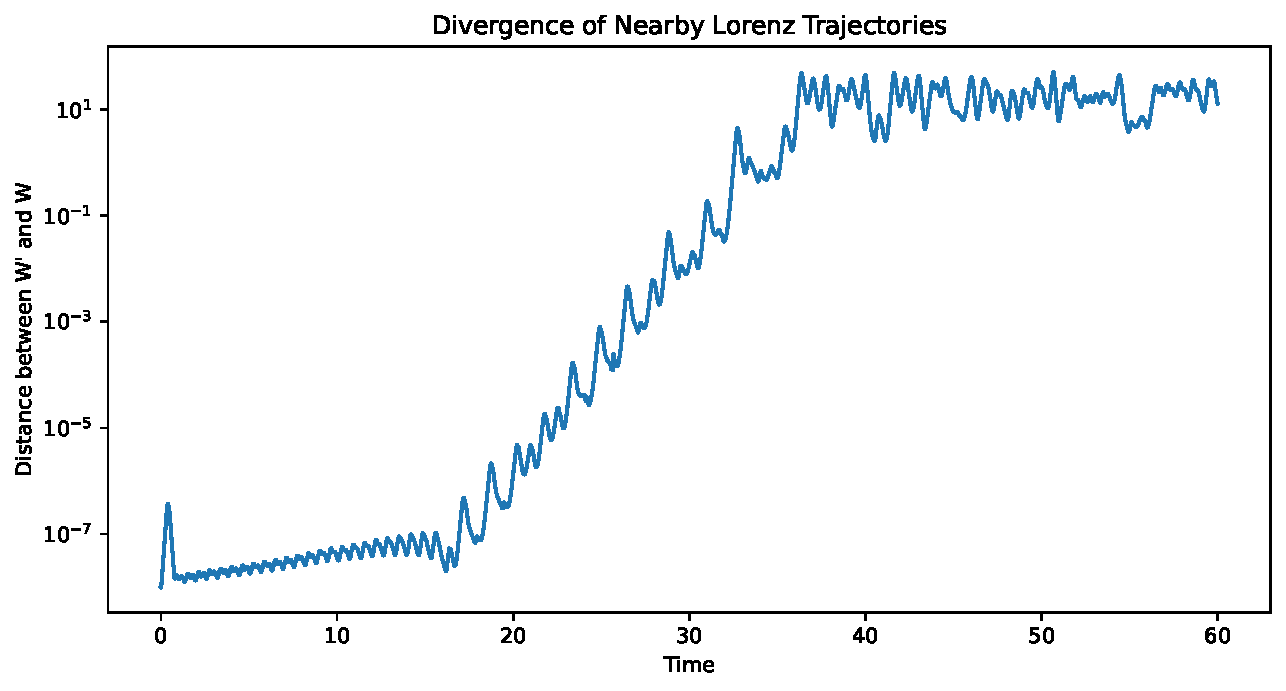
\includegraphics[width=0.8\textwidth]{lorenz_divergence.pdf}
    \caption{Distance between the original and perturbed Lorenz trajectories as a function of time.}
    \label{fig:lorenz_divergence}
\end{figure}

\section{Conclusion}

The Mandelbrot iteration showed that small changes in the complex parameter \(c\)
can strongly affect whether the sequence remains bounded or diverges. Similarly,
the Lorenz system showed sensitive dependence on initial conditions. Two
trajectories starting only \(10^{-8}\) apart eventually separated significantly, which show just how even a little change in the initial conditions of a system can lead to very different evolutions of the system.

\end{document}\begin{figure}
    \centering
    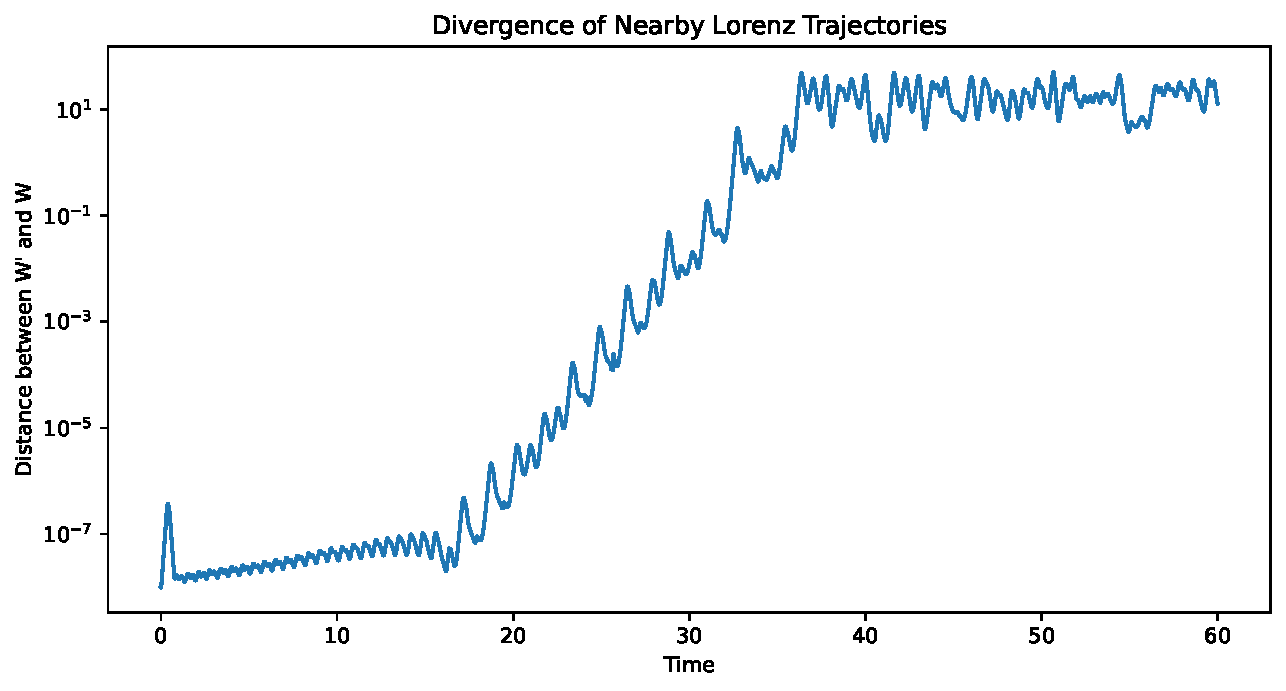
\includegraphics[width=0.5\linewidth]{lorenz_divergence.pdf}
    \caption{Enter Caption}
    \label{fig:placeholder}
\end{figure}
